\documentclass[cits]{PoS}
\usepackage{color,verbatim,amsmath,amssymb}
\usepackage{lineno}

\newcommand{\url}[1]{{\tt #1}}
\newcommand{\lsim}
{\;\raisebox{-.3em}{$\stackrel{\displaystyle <}{\sim}$}\;}
\newcommand{\gsim}
{\;\raisebox{-.3em}{$\stackrel{\displaystyle >}{\sim}$}\;}
\newcommand{\gmt}{\ensuremath{(g-2)_\mu}}
\newcommand{\br}{{\rm BR}}
\newcommand{\bsg}{BR($b \to s \gamma$)}
\newcommand{\btn}{BR($B_u \to \tau \nu_\tau$)}
\newcommand{\kmn}{BR($K \to \mu \nu_\mu$)}
\newcommand{\bmm}{\ensuremath{\br(B_s \to \mu^+\mu^-)}\ }
\newcommand{\ssi}{\ensuremath{\sigma^{\rm SI}_p}}
\newcommand{\ssd}{\ensuremath{\sigma^{\rm SD}_p}}
\newcommand{\Och}{\ensuremath{\Omega_\chi h^2}}
\newcommand{\sweff}{\sin^2\theta_{\mathrm{eff}}}
\newcommand{\MW}{M_W}
\newcommand{\MZ}{M_Z}
\newcommand{\Mh}{M_h}
\newcommand{\MH}{M_H}
\newcommand{\MA}{M_A}
\newcommand{\MHSM}{M_H^{\rm SM}}
\newcommand{\mt}{m_t}
\newcommand{\mgl}{m_{\tilde g}}
\newcommand{\cha}[1]{\tilde \chi^\pm_{#1}}
\newcommand{\champ}[1]{\tilde \chi^\mp_{#1}}
\newcommand{\mcha}[1]{m_{\tilde \chi^\pm_{#1}}}
\newcommand{\neu}[1]{\tilde \chi^0_{#1}}
\newcommand{\mneu}[1]{m_{\tilde \chi^0_{#1}}}
\newcommand{\mste}{m_{\tilde t_1}}
\newcommand{\mstaue}{m_{\staue}}
\newcommand{\staue}{\tilde \tau_1}
\newcommand{\astaue}{\overline{\tilde \tau_1}}
\newcommand{\sel}[1]{e_{#1}}
\newcommand{\asel}[1]{\overline{e_{#1}}}
\newcommand{\tb}{\tan\beta}
\newcommand{\ecm}{\sqrt{s}}
\newcommand{\tev}{\,\, \mathrm{TeV}}
\newcommand{\gev}{\,\, \mathrm{GeV}}
\newcommand{\mev}{\,\, \mathrm{MeV}}
\newcommand{\cmsATLAS}{CMS/ATLAS\ }

\newcommand{\htr}[1]{{\color{red}  #1}}
\newcommand{\htb}[1]{{\color{blue}  #1}}
\newcommand{\htg}[1]{{\color{green}  #1}}
\newcommand{\hto}[1]{{\color{Orange}  #1}}
\newcommand{\htp}[1]{{\color{Purple}  #1}} \newcommand{\delr}[1]{\htr{\st{#1}}}
\newcommand{\delb}[1]{\htb{\st{#1}}}
\newcommand{\delg}[1]{\htg{\st{#1}}}
\newcommand{\delo}[1]{\hto{\st{#1}}}
\newcommand{\delp}[1]{\htp{\st{#1}}}

\newcommand{\ETslash}{/ \hspace{-.8em}\ensuremath{E_T}\ }
\newcommand{\pTslash}{/ \hspace{-.8em}\ensuremath{p_T}}

\title{Global SUSY Fits with the MasterCode Framework COLLABORATION}

\ShortTitle{Global SUSY Fits with the MasterCode Framework COLLABORATION}

\author{\speaker{Samuel ROGERSON}%
         %\thanks{A footnote may follow.}\\
        Imperial College London\\
        E-mail: \email{samr@cern.ch}}

%\author{Another Author\\
%        Affiliation\\
%        E-mail: \email{...}}

\abstract{We present the latest results of the MasterCode collaboration on
global SUSY fits. Currently available experimental data are used to determine
the preferred SUSY and Higgs boson mass scales. The data comprise a combination
of high-energy SUSY searches, low-energy precision measurements and
astrophysical data. We include all relevant LHC searches for SUSY, electroweak
precision observables such as the W boson mass and the anomalous magnetic moment
of the muon, B physics observables such as \bsg, as well as the cold
dark matter density in the Universe. The preferred masses for SUSY particles as
well as for the MSSM Higgs bosons are derived in the context of four GUT-based
realizations of the MSSM. We find a preference for relatively light SUSY masses,
which the direct searches at the LHC shift to slightly higher mass scales. The
preferred mass values can directly be compared to the reach of the LHC and
future $e^{+}e^{-}$ colliders as well as to current and future direct detection searches
for dark matter. }

\FullConference{XXIst International Europhysics Conference on High Energy Physics\\
                 21-27 July 2011\\
                 Grenoble, Rh\^ones Alpes France}

\begin{document}

\section{Introduction}
We extend our previous\cite{mc5} frequentist analyses of the CMSSM, NUHM1, VCMSSM and mSUGRA parameter
spaces taking into account all the public results of searches for supersymmetry using data
from the 2010 LHC run and the Xenon100 direct search for dark matter scattering. The LHC 
data set includes ATLAS and CMS searches for jets $+$ \ETslash events (with or without 
leptons) and for the heavier MSSM Higgs bosons, and the upper limit on
\bmm including data from LHCb as well as CDF
and D\O .

\section{Experimental Results}
\subsection{ATLAS and CMS}
We incorporate the CMS~ \ETslash\cite{MHT} and the ATLAS $0\ell$ and $1\ell$~\cite{ATLAScombined}
results, each using $\sim 35pb^{-1}$ of data. The limits obtained
in both searches are very close to the median expected limit, corresponding 
to a difference between the numbers of events observed and expected from
background that is negligible compared to the $\sigma_{eff}$ for the number of 
background events. We therefore approximate the impact of these searches outside
their nominal 95\% CL contour by assuming that the number of effective $\sigma$ 
is simply proportional to the number of signal events expected at any given
supersymmetric point, which we assume to be $\sim M^{-4}$ and we then
calculate the corresponding $\chi^{2}$ penalty as
\begin{equation}
    \chi^{2}_{p} = \chi^{2}_{95\%}\left(\frac{M_{p}}{M_{95\%}}\right)^{4}
\end{equation}
For each point in parameter space, we take the contribution arising from the
search with the maximum \emph{expected} exclusion.

\subsection{Heavy Higgs}
The CMS Collaboration has provided model-independent limits on the H/A
production cross section times $\tau^{+}\tau^{-}$ branching ratio $(\sigma\times
BR)$at the 68\%, 95\% and 99.7\% $CL_{s}$ as functions of $M_{A}$~\cite{nikitenko}, corresponding 
to a one-dimensional $\chi^{2}$ contribution of 1, 3.84, and 9, respectively. For 
each fixed value of $M_{A}$ , we assume that the $\chi^{2}$ penalty for other values of
$\sigma\times BR$ may be approximated by the functional form 
$\Delta\chi{2}\propto (\sigma\times BR)^{p(M_{A})}$, normalized to unity on the 
68\% CL line and fitting the power $p(M_{A})$ independently for each value of
$M_{A}$ (typical values are $\sim 1.3$). Assuming a scaling law of
$\left(\sigma\times BR\right)\propto \tan^{2}\beta$, we then apply a $\chi^{2}$ penalty 
calculated as
\begin{equation}
    \chi^{2}\sim\left(\frac{\tan^{2}\beta}{\tan^{2}\beta_{95\%}} \right)^{p\left(M_{A}\right)}
\end{equation}

\subsection{\bmm}
The paper by LHCb~\cite{lhcb-bmm} provides 95\% and 90\% upper limits on
\bmm\ of 56 and $43 \times 10^{-9}$,
to be compared with the Standard Model prediction of
$(3.2 \pm 0.2) \times 10^{-9}$.
A combination of these with the results provided by CDF~\cite{cdf-bmm} and D\O~\cite{d0-bmm}
is achieved by first performing approximate studies, based on the signal and background expectations in each experiment, and comparing
with the observed pattern of events, generating toy experiments that reproduce their quoted 90\% CL upper limits.
The toy LHCb experiment was constructed using the information shown in Table~3 of~\cite{lhcb-bmm}.
The toy CDF experiment was based on the information given in Table II of~\cite{cdf-bmm},
combined with the invariant mass resolution, normalization factors and averaged 
Neural Network efficiencies quoted in the text. 
Finally, the toy D\O\ experiment was based on Fig.~4 of~\cite{d0-bmm}, together with
the invariant mass resolution and normalization factor quoted in the text.
The results of the three experiments were combined using the $CL_{s}$ method.
Our global fit uses the full likelihood function calculated using the above
experimental information to beyond the 99\% CL.

\subsection{Xenon100 search for dark matter scattering}
Finally, we implement the constraint imposed by the direct upper limit
on dark matter scattering given by the Xenon100 experiment~\cite{Xenon100new}. 
This takes the form of a 95\% CL upper limit on the spin-independent cross section as a function of $\mneu{1}$. 
The Xenon100 Collaboration report the observation of 3 events where $1.8 \pm 0.6$ events were expected.
Using Poisson statistics with a non-negligible background,
we have constructed a model for the Xenon100 contribution to the
global $\chi^2$ likelihood function as a function of the number of events using the $CL_s$ method.
This turns out to be quite similar to a Gaussian function with mean 1.2 and standard deviation 3.2 events.
Our model for the Xenon100 likelihood function yields a 90\% CL upper limit of 6.1 events so,
for any given value of $\mneu{1}$, we assume that the 90\% CL upper limit on
$\ssi$ quoted in~\cite{Xenon100new} corresponds to 6.1 events,
and use simple scaling to estimate the event numbers corresponding to other values of $\ssi$.
We then use the Gaussian model for the Xenon100 $\chi^2$ function to estimate the
contribution of this experiment to the global likelihood function for other $\ssi$ values.
We note that, because of the insignificant `excess' of 1.2 events in the Xenon100 data,
there is a contribution $\Delta \chi^2 \sim 0.3$ to the global likelihood function
at small values of \ssi~%

We take account of the uncertainty in the calculation of $\ssi$  
induced principally by the experimental uncertainty in the $\pi$-nucleon
$\sigma$ term, $\Sigma_{\pi N}$.
Estimates of $\Sigma_{\pi N}$ up to a value as large as 
$64 \pm 8 \mev$ have been given in the literature~\cite{Pavan:2001wz}.
Here we span the plausible range by using as our default $\Sigma_{\pi N} = 50 \pm 14 \mev$, while
also showing some results for $\Sigma_{\pi N} = 64 \pm 8 \mev$~%

\section{Results}
We see that for the constrained models of supersymmetry considered, the direct
searches from \cmsATLAS push the best fit points, Table \ref{tab:bf}, in $m_{1/2}$ to $\sim 500\gev$
corresponding to $m_{\tilde{g}}\gsim1\tev$. The CMS limits on heavy Higgs
production and our compilation of LHCb, CDF and D\O\ constraints on \bmm have
impacts on the parameter spaces of the NUHM1, but do not affect significantly 
the favoured regions of the CMSSM, VCMSSM and mSUGRA.
The Xenon100 results have an impact on the model parameter spaces that would be significant
if $\Sigma_{\pi n}$ were large,$\sim60\mev$. However, the current uncertainty in
$\Sigma_{\pi n}$ does not permit a strong conclusion to be drawn.

Overall, we calculate probabilities in the constrained models after the search
exclusions of $<20\%$, Table \ref{tab:bf} and Figure \ref{fig:m0m12pval}. With the
advent of direct searches using $1fb^{-1}$ of data one might expect to see
$p<5\%$ if no signal is seen.  This not only applies to direct searches using 
\ETslash with (or without) leptons, but also the indirect searches through processes 
like \bmm where these models have preferred values $\sim\ $SM.

This indicates a slight tension in these models between the preference for rather light colour-neutral states
arising in particular from $(g-2)_{\mu}$ and the search limits from the direct searches for coloured SUSY
particles at the LHC. The mSUGRA scenario yields a significantly worse description of the data
than the other considered models already for the pre-LHC data set, and inclusion of the 2010 LHC
and Xenon100 constraints has only a small impact on the preferred fit values and the fit probabilities. 
If the upcoming LHC results lead to a further increase of the excluded mass regions for coloured superpartners,
the CMSSM, NUHM1 and VCMSSM scenarios could eventually get under pressure. Such a tension could be avoided in
realisations of SUSY with a larger splitting between the coloured and the colour-neutral part of the spectrum 
(for instance in GMSB-type scenarios), such that the masses of squarks and gluinos are in the $\tev$ range, 
while sleptons, neutralinos and charginos can still be light.


\begin{table*}[htb!]
    \begin{center}
        \begin{tabular}{|r||c|c|c|c|c|c||c|}
          \hline
          Model & Min $\chi^{2}$ & Prob & $m_{1/2}$ & $m_{0}$ & $A_{0}$ &
          $\tan\left(\beta\right)$ & $M_{h}^{\textrm{no LEP}}$  \\
          \hline\hline
          \textcolor{red}{CMSSM} & 22.5/19 & 26\% & 310 & 60 & -60 & 10 & 109 \\
           post-LHC/Xenon & 26.2/20 & 16\% & 470 & 170 & -780 & 22 & 116 \\
          \hline  
          \textcolor{red}{NUHM1} & 20.5/17 & 25\% & 240 & 100 & 920 & 7 & 119 \\
           post-LHC/Xenon & 24.2/19 & 19\% & 530 & 110 & -370 & 27 & 118 \\
          \hline
        \end{tabular}
    \end{center}
    \caption{\it 
        The best fit values of the four models considered
        }
    \label{tab:bf}
\end{table*}

\begin{figure*}[htb!]
    \resizebox{8.3cm}{!}{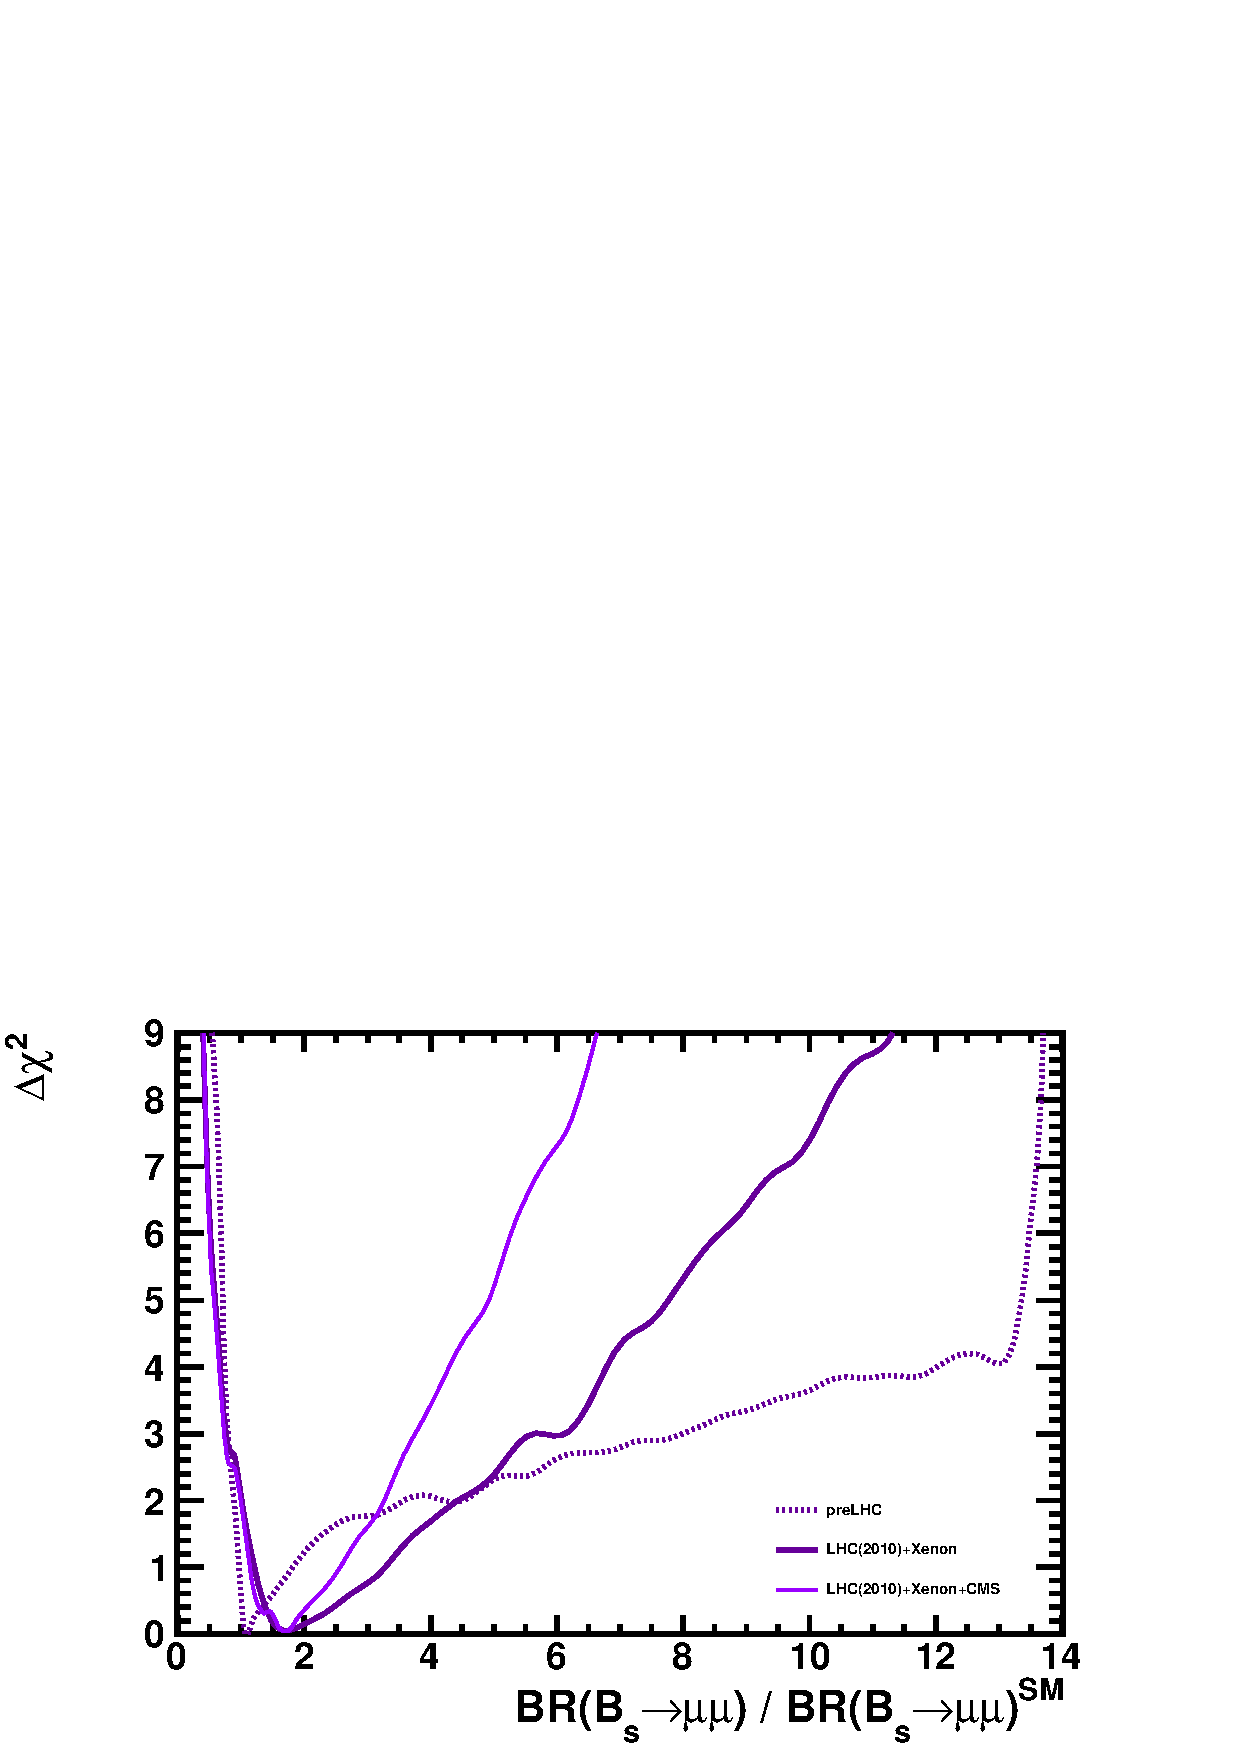
\includegraphics{nuhm1.pdf}}
    \resizebox{8.3cm}{!}{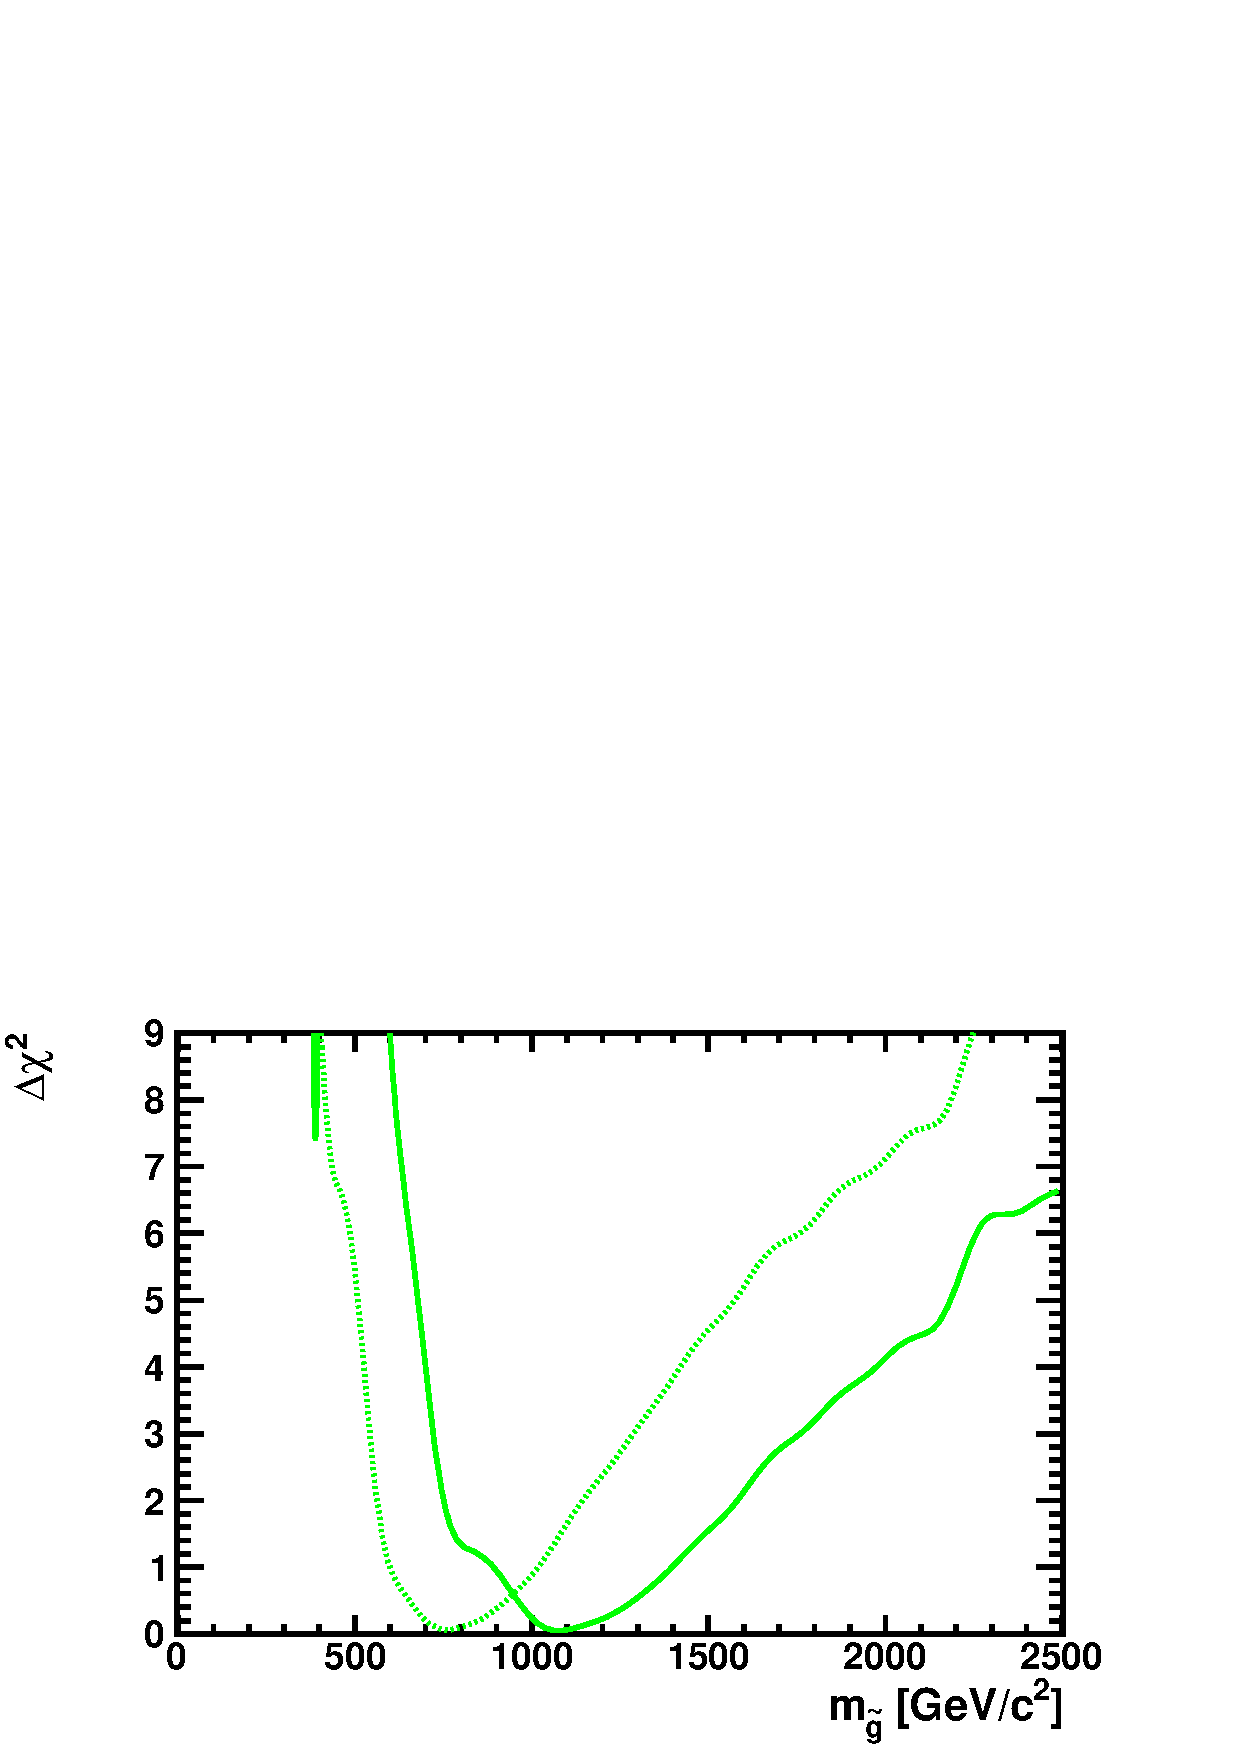
\includegraphics{cmssm.pdf}}
    \vspace{-1cm}
    \caption{\it 
        The ($m_{0}$ , $m_{1/2}$ ) planes in the NUHM1 (left) and the CMSSM (right), for the
        after applying the various experimental constraints. In each plane, different regions are
        colour-coded according to the p-values found in our global fits. We note that
        in the LHC$_{2010}$ analysis the regions with $p > 0.05$ extend up to
        $m_{1/2} \sim 1500 \gev$ and $2000 \gev$ respectively
    }
    \label{fig:m0m12pval}
\end{figure*}

\clearpage

\begin{thebibliography}{99}
\bibitem{mc5}
  O.~Buchmueller {\it et al.},
  Eur.\ Phys.\ J.\  C {\bf 71} (2011) 1634
  [arXiv:1102.4585 [hep-ph]].
  %%CITATION = EPHJA,C71,1634;%%

\bibitem{MHT}
V.~Khachatryan {\it et al.} [CMS Collaboration],
{\tt http://cdsweb.cern.ch/record/1343076/}
{\tt files/SUS-10-005-pas.pdf};
see also \\
{\tt https://twiki.cern.ch/twiki/bin/view/}
{\tt CMSPublic/PhysicsResultsSUS}.

\bibitem{ATLAScombined}
G.~Aad {\it et al.} [ATLAS Collaboration],
{\tt http://cdsweb.cern.ch/record/1345745/} {\tt files/ATLAS-CONF-2011-064.pdf},
{\tt https://atlas.web.cern.ch/Atlas/GROUPS/} {\tt PHYSICS/CONFNOTES/ATLAS-CONF-2011-064/}.

\bibitem{nikitenko} V.~Khachatryan {\it et al.} [CMS Collaboration],
{\tt https://twiki.cern.ch/twiki/bin/view/} {\tt CMSPublic/PhysicsResultsHIG10002}/


\bibitem{lhcb-bmm} R.~Aaij {\it et al.}  [LHCb Collaboration],
  arXiv:1103.2465 [hep-ex].
  %%CITATION = ARXIV:1103.2465;%%

\bibitem{cdf-bmm} T.~Aaltonen {\it et al.}  [CDF Collaboration],
  Phys.\ Rev.\ Lett.\  {\bf 100}, 101802 (2008)
  [arXiv:0712.1708 [hep-ex]]; see also
  %%CITATION = PRLTA,100,101802;%%
{\tt http://www-cdf.fnal.gov/physics/new/}
{\tt bottom/090813.blessed-Bsd2mumu//}
{\tt bsmumupub3.7fb$\underline{~}$v01.pdf}.

\bibitem{d0-bmm} V.~M.~Abazov {\it et al.}  [D0 Collaboration],
  Phys.\ Lett.\  B {\bf 693} (2010) 539 
  [arXiv:1006.3469 [hep-ex]].
  %%CITATION = PHLTA,B693,539;%%

\bibitem{Xenon100new}
E.~Aprile {\it et al.}  [XENON100 Collaboration],
  arXiv:1104.2549 [astro-ph.CO].
  %%CITATION = ARXIV:1104.2549;%%

\bibitem{Pavan:2001wz}
M.~M.~Pavan, I.~I.~Strakovsky, R.~L.~Workman and R.~A.~Arndt,
PiN Newslett.\  {\bf 16} (2002) 110 
[arXiv:hep-ph/0111066].
%%CITATION = 00076,16,110;%%
\end{thebibliography}

\end{document}
